\section{Laser Thermal Control}
	\label{mtLSRthermal}
The functioning of the optical payload is dependent on a specific temperature interval, so in order to be able to meet the top level requirements, thermal control considerations for the emitter and receiver should be taken into account. 

\subsection{Thermal Physics}
	\label{mtLSRthermalphysics}
Two important mechanisms of thermal conductivity are (free) electron translation (crystal momentum) and phonon states. A phonon (state) is a quantum of acoustic energy, analogous to the quantum of electromagnetic radiation, the photon. Thermal excitations in a crystal or in an elastic medium can be described as a population of phonons. Basically, phonons represent a mode of vibration occurring in a rigid crystal lattice. Since, on one side, individual electrons in a crystal lattice are bound in terms of quantisized energy levels and on the other side they are interconnected to neighboring particles by electric force (attraction or repulsion) as a function of distance, in most solids the energy given to lattice vibrations is the dominant contribution to the heat capacity, i.e. induced thermal energy is converted to a change in rate of crystal momentum or phonon state, which can be represented by a difference in internal energy. In this light, the terms 'thermal energy' and 'internal energy' represent the same quantity. 

From an electron point of view, a change in temperature (or any change in state variable) represents the quest for a new thermal equilibrium situation. Since electrons are fermions, their orbit population is described by the temperature dependent Fermi-Dirac distribution. Fermions show the tendency to occupy the lowest energy levels and since they are limited due to Pauli's exclusion principle, which states no identical fermion with equal intrinsic spin can occupy the same energetic orbit, not every electron can be in the ground state. Increasing the internal energy will therefor represent thermal excitation.  

\subsection{Theoretical Thermal Limits For Lasers}
	\subsubsection{Gain Medium Thermal Overloading}
		\label{mtLSRthermaloverload}	
Thermal overloading can be divided to the temperature interval at which electron excitation is impossible and the interval at which permanent crystal lattice deformation occurs.

\textit{Short term temperature increase (T < 323.15K)}
To begin with the first phenomenon, in order to excite any electron, the conduction band should not be completely filled in thermal equilibrium. Any excitation, so also stimulated excitation, would be impossible and hence no lasing action would occur. In the real world, a small part of the electrons will give rise to stimulated emission since not all electrons would occupy the highest energy bands, considering the temperature to increase. However, population inversion would not be present. If the temperature is decreased afterwards, the gain material would be able to provide lasing action, making it an short-term problem with no permanent significance. 

\textit{Long term temperature increase (T > 323.15K)}
However, if the induced (thermal) energy is increased even further, the crystal lattice can eventually alter in time. This crystal lattice deformation not only implies the gain material, but all optical subparts, causing possible lasing failure. Recrystallization of the material can occur if the upper limit of the temperature interval is reached, giving birth to long-term (partial) failure. Another longterm effect is thermal fatigue for parts within the laser.

	\subsubsection{Thermal Lensing}
		\label{mtLSRthermallensing}
		
\textit{Long term temperature increase (T > 303.15K)}
Particularly in high-power lasers, the appearance of a temperature-gradient in the gain medium often causes a significant 'thermal lens'. The gain medium has higher internal energy on the beam axis, typically causing some transverse gradient of the refractive index according to the temperature-dependent Sellmeier equation. 

\begin{figure} [ht]
	\begin{center}
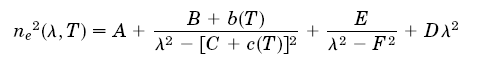
\includegraphics[scale=1]{chapters/img/TISE.png}	
\caption{Refractive index as function of radial position, where the Sellmeier coefficients A, B, C, D, E, and F are constants dependent on gain material, c and b are temperature dependent, T is the temperature in degrees centigrade, and l is the wavelength in micrometers.}
\label{thermal_lensing}
\end{center}
\end{figure}

Thermal lensing occurs due to the combined effect of the thermal expansion and thermally induced refractive index change. The magnitude of the thermal lensing scales proportional to the power absorbed by the gain medium and the thermo-optic coefficient of the material, and inversely proportional to the thermal conductivity of the material. 

The Sellmeiser equation could also be used for the change in refractive index for all other optical subparts in the laser, like the lenses. Since the refractive index will change due to the change in temperature, this has to be taken into account.   

\begin{figure} [ht]
	\begin{center}
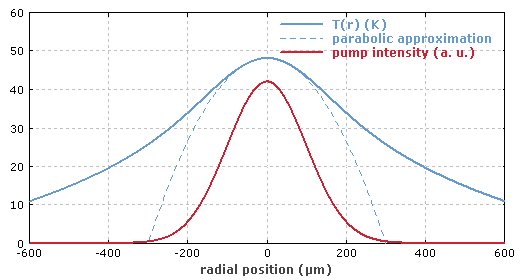
\includegraphics[scale=1]{chapters/img/thermal_lensing.png}	
\caption{Transverse pump intensity distribution (red) and thermal profile (blue). The temperature profile is approximately parabolic only near the center of the crystal.}
\label{thermal_lensing}
\end{center}
\end{figure}

External induced thermal energy can therefor cause the formation of a thermal lens, causing the beam quality to alter. Especially beam divergence tends to decrease by the formation of a thermal lens, i.e. the change in refractive index change per unit temperature (dn/dT) should be kept within limits. The absence of thermal control can even lead to non-localized thermal lensing, since temperature-gradients can be localized away from the principal axes. 
			
	\subsubsection{Multi-Phonon Transitions}
		\label{mtLSRphonon}
\textit{Long term temperature increase (T > 353.15K)}
The upper-state lifetime (the lifetime of the population of the upper laser level) can be strongly reduced by decay processes which involve the simultaneous emission of multiple phonons. Multiple phonons are typically required for such transitions because the energy of a single phonon is not sufficient to match the difference in level energies. The rate of multi-phonon transitions decreases with the increasing number of phonons required. Temperature-gradients can influence the phonon transition and hence influence the the upper-state lifetime, decreasing the beam quality. 

	\subsubsection{Dielectric Transmission}
		\label{mtLSRditrans}
\textit{Long term temperature increase (T > 313.15K)}
Optically absorbing layers (dielectric transmission decrease) can form on the exit face of the fully reflective mirror and on the doubling crystal, resulting in a decay of output power. The absorbed optical energy creates thermal gradients with which affects phase matching and hence lowering the beam quality. 

	\subsubsection{Limit in Electron Movement}
		\label{mtLSRelecmovement}
\textit{Long term temperature decrease (T < 273.15K)}
If the internal energy decreases to much, the exciton dynamics would alter, i.e. electrons will not be able to be excited to higher energy levels. This temperature dependent tendency is caused by the Boltzmann distribution, giving rise to an increase of potential energy at the lowest energy level. 

\subsection{Thermal Control}
	\label{mtLSRthermalcontrol}
As seen in the previous paragraphs, the temperature interval for proper lasing action roughly equals 273.15 < T [K] < 313.15. Since the thermal environmnent is extremely harsh (extremely cold background temperature, intense solar radiation, sudden loss of temperature in shadow and the presence of vacuum), thermal control considerations should be taken into account. 

